\documentclass[12pt, a4paper, openany, oneside]{report}
\usepackage{emptypage}
\usepackage[square,numbers]{natbib}

\newcommand{\rupee}{Rs.~}

\usepackage{makecell}
\usepackage{float}
\usepackage{booktabs}
\usepackage{afterpage}
\usepackage{hyperref}
\usepackage{tabularx}
\usepackage{xltabular}
\hypersetup{
    colorlinks=true,
    linkcolor=black,
    urlcolor=black,
    breaklinks=false,
    citecolor=black,
}

\usepackage[nottoc,notlof,notlot]{tocbibind}
\usepackage{framed}
\usepackage{graphicx}
\usepackage{caption}
\captionsetup[table]{skip=10pt}
\usepackage[utf8]{inputenc}
\usepackage{amsmath}
\usepackage{setspace}
\usepackage[english]{babel}
\usepackage{pbox}
\usepackage{url}
\usepackage{array}
\usepackage{amssymb}
\usepackage{ragged2e}
\usepackage{sectsty}
\usepackage{soul}
\usepackage{chngcntr}
\usepackage{multirow}
\usepackage{enumitem}

\providecommand{\keywords}[1]{\textbf{\textit{Keywords:}} #1}
\textwidth 161mm
\textheight 230mm
\linespread{1}
\usepackage{titlesec}
\chapterfont{\centering}
\newcolumntype{P}[1]{>{\centering\arraybackslash}p{#1}}
\newcolumntype{M}[1]{>{\centering\arraybackslash}m{#1}}
\renewcommand{\baselinestretch}{1.3}

\titleformat{\chapter}[display]
{\normalfont\huge\bfseries\centering}{\chaptertitlename\ \thechapter}{10pt}{\Huge\centering}
\titlespacing*{\chapter}{0pt}{-50pt}{10pt}

\usepackage[
  top    = 1.2in,
  bottom = 1in,
  left   = 1.3in,
  right  = 1in,
]{geometry}

% ── colour boxes for examples ──────────────────────────────────────────
\usepackage{tcolorbox}
\tcbuselibrary{skins,breakable}

\newtcolorbox{examplebox}[1][]{
  breakable, enhanced,
  colback=blue!4!white, colframe=blue!40!black,
  fonttitle=\bfseries, title=Example — #1,
  left=6pt, right=6pt, top=4pt, bottom=4pt
}

\newtcolorbox{gapbox}{
  breakable, enhanced,
  colback=red!4!white, colframe=red!50!black,
  fonttitle=\bfseries, title=Competitive Gap,
  left=6pt, right=6pt, top=4pt, bottom=4pt
}

\newtcolorbox{valuebox}{
  breakable, enhanced,
  colback=green!4!white, colframe=green!50!black,
  fonttitle=\bfseries, title=User Value,
  left=6pt, right=6pt, top=4pt, bottom=4pt
}
% ───────────────────────────────────────────────────────────────────────

\begin{document}
\counterwithin{table}{chapter}
\counterwithin{figure}{chapter}
\pagenumbering{gobble}
\thispagestyle{empty}

% =====================================================================
%  TITLE PAGE
% =====================================================================
\begin{center}
Major Project (IT898) Report on \\[0.4em]
\textbf{\Large FUNCTIONAL REQUIREMENTS AND COMPETITIVE DIFFERENTIATORS\\[0.2em]
FOR AN AGENTIC AI INTELLIGENT PORTFOLIO CREATION APPLICATION}\\[1.5em]
Submitted in partial fulfillment of the requirements for the degree of\\[0.3em]
MASTER OF TECHNOLOGY \\
in\\
INFORMATION TECHNOLOGY\\[1.5em]
by \\[0.2em]
\large\textbf{ANKUR PATEL} \\
\textbf{(252IT004)}\\[1em]
\large\textit{under the guidance of} \\[0.2em]
\large\textbf{Dr.\ Biju R Mohan}\\[1em]
\begin{figure}[h]
  \centering
  \includegraphics[width=4cm, height=4cm]{NITKLogo.jpeg}
\end{figure}
\vspace{0.2em}
{\fontsize{13}{13}\selectfont DEPARTMENT OF INFORMATION TECHNOLOGY}\\
{\fontsize{13}{13}\selectfont NATIONAL INSTITUTE OF TECHNOLOGY KARNATAKA, SURATHKAL}\\
{\fontsize{13}{13}\selectfont MANGALORE -- 575025}\\[0.5em]
September 2026
\end{center}

\clearpage
\newpage

% =====================================================================
%  ABSTRACT
% =====================================================================
\thispagestyle{plain}
\begin{center}
\textbf{{\Large ABSTRACT}}\\[0.5em]
\end{center}

The Indian retail investment market is growing rapidly, yet most retail investors face a critical problem: existing portfolio management applications operate as opaque ``black boxes'' -- they deliver recommendations without explaining the reasoning behind them. Platforms such as Jarvis Invest, Savart, Wright Research, Univest, smallcase, and Motilal Oswal IAP offer AI-based personalised portfolios, but none of them expose the complete, traceable workflow connecting the investor's goals to the final portfolio weights.

This report presents a comprehensive Functional Requirements Specification for a novel Agentic AI application designed to bridge this transparency gap. The application is organised around twenty functional requirements: ten core requirements that meet market baseline expectations and ten differentiating requirements that are not provided by any current Indian competitor in an integrated, transparent form.

Every requirement is supported by concrete competitive evidence from a September 2026 deep-dive analysis of seven major Indian portfolio platforms. Each requirement includes a plain-English description, a concrete real-world example, the exact competitive gap it addresses, and an explanation of where in the user's journey it provides value.

\vspace{0.8em}
\keywords{Agentic AI, Functional Requirements, Portfolio Management, LangGraph, Explainability, Reasoning Trace, Competitive Intelligence, India, Retail Investor, Transparency, MFKG, M-SAEA}

\clearpage
\newpage

% =====================================================================
%  TABLE OF CONTENTS
% =====================================================================
\renewcommand*{\contentsname}{\MakeUppercase{Contents}}
\renewcommand*{\listtablename}{\MakeUppercase{List of Tables}}
\renewcommand{\bibname}{REFERENCES}
\thispagestyle{plain}
\pagenumbering{roman}
\setcounter{page}{1}
\addtocontents{toc}{\protect\thispagestyle{plain}}
\tableofcontents
\cleardoublepage

\listoftables
\addcontentsline{toc}{chapter}{LIST OF TABLES}
\cleardoublepage

% =====================================================================
%  ABBREVIATIONS
% =====================================================================
\begin{center}
\textbf{{\huge ABBREVIATIONS}}
\addcontentsline{toc}{chapter}{ABBREVIATIONS}
\vspace{0.5cm}
\begin{tabbing}
    \hspace*{4.5cm} \= \kill
    AI          \> Artificial Intelligence \\
    LLM         \> Large Language Model \\
    NLP         \> Natural Language Processing \\
    MFKG        \> Mutual Fund Knowledge Graph \\
    RAG         \> Retrieval-Augmented Generation \\
    GraphRAG    \> Graph-based Retrieval-Augmented Generation \\
    M-SAEA      \> Multi-agent Safety and Audit Extension Architecture \\
    SEBI        \> Securities and Exchange Board of India \\
    VIX         \> Volatility Index \\
    RMS         \> Risk Management System \\
    AMFI        \> Association of Mutual Funds in India \\
    STCG        \> Short-Term Capital Gains \\
    LTCG        \> Long-Term Capital Gains \\
    SIP         \> Systematic Investment Plan \\
    PMS         \> Portfolio Management Services \\
    RIA         \> Registered Investment Adviser \\
    SEBI IA     \> SEBI-registered Investment Adviser \\
    SEBI RA     \> SEBI-registered Research Analyst \\
    AUA         \> Assets Under Advisory \\
    AUM         \> Assets Under Management \\
    ROE         \> Return on Equity \\
    VaR         \> Value at Risk \\
    CAGR        \> Compound Annual Growth Rate \\
    MVP         \> Minimum Viable Product \\
    FR-C        \> Functional Requirement -- Core \\
    FR-D        \> Functional Requirement -- Differentiating \\
    ESG         \> Environmental, Social, and Governance \\
    FMCG        \> Fast-Moving Consumer Goods \\
\end{tabbing}
\end{center}
\cleardoublepage

% =====================================================================
%  CHAPTER 1: INTRODUCTION
% =====================================================================
\pagenumbering{arabic}
\setcounter{page}{1}

\chapter{Introduction}

\section{The Problem with Today's Portfolio Apps}

The Indian retail equity market has grown dramatically. According to AMFI data, unique mutual fund investors crossed 5 crore in 2025, and demat accounts at NSE and BSE crossed 17 crore by mid-2026. Despite this growth, most retail investors do not receive the kind of personalised, transparent financial advice that institutional investors take for granted.

Several technology platforms have emerged to address this gap: smallcase, Univest, Motilal Oswal IAP, Savart, Wright Research, and Jarvis Invest. Each offers some form of portfolio creation, stock selection, risk profiling, and rebalancing. However, a September 2026 deep-dive competitive analysis of all seven platforms reveals a consistent and critical gap:

\begin{framed}
\textit{``Existing platforms cover many parts of portfolio creation and management, including screening, personalisation, portfolio analysis, risk monitoring and rebalancing. However, the level of transparency differs across products, and the complete connection between the investor's inputs, the data used, the recommendation, the portfolio weight and the resulting portfolio change is not consistently exposed in one traceable workflow.''}
\end{framed}

In plain terms: every existing app tells the investor \textbf{what} to buy. None of them properly explain \textbf{why}.

\section{An Analogy}

Imagine visiting a doctor who prescribes three medicines after examining you, but refuses to explain:
\begin{itemize}
  \item Why these three medicines, and not two or four?
  \item Why this dosage and not a different one?
  \item What are the risks if you combine them?
  \item What happens if your condition changes?
\end{itemize}

You would not trust that doctor. Yet every Indian portfolio application does precisely this. They say ``Buy 10\% HDFC Bank, 8\% Infosys, 7\% Cipla'' and expect the investor to comply without explanation. Our application is built to be the doctor who explains every single decision.


\section{Structure of This Report}

\begin{itemize}
  \item \textbf{Chapter 2} -- The competitive landscape: who the competitors are and what they actually offer.
  \item \textbf{Chapter 3} -- Core Functional Requirements (FR-C01 to FR-C10): the baseline every good app must meet.
  \item \textbf{Chapter 4} -- Differentiating Functional Requirements (FR-D01 to FR-D10): what no competitor currently does.
  \item \textbf{Chapter 5} -- Requirements summary, pipeline, and design thesis.
  \item \textbf{Chapter 6} -- Data requirements.
\end{itemize}

% =====================================================================
%  CHAPTER 2: MARKET CONTEXT
% =====================================================================
\chapter{Market Context and Competitive Landscape}

\section{The Seven Platforms}

\begin{table}[H]
\centering
\caption{Competitor Classification (September 2026 Deep Research)}
\label{tab:competitors}
\begin{tabularx}{\textwidth}{|l|X|l|}
\hline
\textbf{Platform} & \textbf{Primary Role} & \textbf{Classification} \\
\hline
smallcase & Model-portfolio marketplace + broker infrastructure & Direct \\
Univest & Research + advisory + brokerage + portfolio review & Direct \\
Motilal Oswal IAP & Pre-packaged advisory portfolios via RIAs & Direct product \\
Savart & Personalised AI advisory + PMS & Direct \\
Wright Research & Quant/factor portfolios + diagnostics + PMS & Direct \\
Jarvis Invest & AI-personalised portfolio + 24/7 risk management & Direct \\
MarketSenseAI & Multi-agent AI for professionals (S\&P 500/100) & Tech benchmark \\
\hline
\end{tabularx}
\end{table}

\section{Key Facts Per Competitor}

\textbf{smallcase} (CASE Platforms Pvt.\ Ltd.): Primarily a technology provider -- not an advisor. Offers themed stock/ETF baskets created by SEBI-registered managers. Recently added Wealth Office AI. Key limitation: no universal financial-planning questionnaire; the Investment Score is rule-driven and not personalised.

\textbf{Univest}: Integrates stock research, advisory, portfolio review, and brokerage. AI tools do preliminary stock screening, but a SEBI-registered human analyst validates every recommendation. This is explicitly documented in its legal terms. General insights do not account for individual risk tolerance.

\textbf{Motilal Oswal IAP}: Pre-packaged equity portfolios. Investors cannot customise an IAP -- only accept or reject the entire order, not individual stocks. No financial planning questionnaire documented. IAP-specific client count and AUA are not publicly disclosed.

\textbf{Savart}: Personalised Portfolio-on-Demand using APART AI (three layers: Quant, IRIS, Synapse). Scale: 4 lakh+ users, \rupee4,500 crore AUA. Exact model architecture and training data are not publicly disclosed.

\textbf{Wright Research}: Uses 300+ quantitative factors across ten groups. ML models for market-regime modelling. Portfolio diagnostic tools are the most detailed of any Indian competitor. Exact architecture undisclosed.

\textbf{Jarvis Invest}: Personalised equity portfolios with a 24/7 Risk Management System (RMS). Scale: approximately 70,000 investors, \rupee1,500 crore AUA. 32+ broker partners. Training dataset and architecture undisclosed.

\textbf{MarketSenseAI} (Alpha Tensor Technologies): The only competitor with a publicly documented multi-agent LLM architecture (News, Fundamentals, Dynamics, Macro $\rightarrow$ Synthesis). Targets financial professionals and global equities -- not Indian retail investors. Classified as an adjacent technology benchmark.

\section{What Is Already Common -- And Therefore Not a Differentiator}

\begin{table}[H]
\centering
\caption{Features Already Standard Across Most Competitors}
\label{tab:common}
\begin{tabularx}{\textwidth}{|X|l|}
\hline
\textbf{Feature} & \textbf{Present In} \\
\hline
Risk profiling & Univest, Savart, Wright, Jarvis \\
Personalised portfolio generation & Savart, Wright, Jarvis, Univest \\
Portfolio tracking and monitoring & All six direct competitors \\
Rebalancing (automated or manual) & All six direct competitors \\
Stock screening and filtering & Univest, Wright, Jarvis \\
Broker integration and execution & smallcase, Univest, Jarvis \\
Financial goal planning & Univest, Savart, Wright, Jarvis \\
AI or quant-based stock analysis & Univest, Savart, Wright, Jarvis \\
\hline
\end{tabularx}
\end{table}

Claiming only these features is \textbf{insufficient}. They are market expectations, not differentiators.

% =====================================================================
%  CHAPTER 3: CORE FUNCTIONAL REQUIREMENTS
% =====================================================================
\chapter{Core Functional Requirements}

Core requirements are the baseline capabilities every credible portfolio application must provide. Without them, the application is not competitive. They are implemented in the Minimum Viable Product (MVP).

% ─────────────────────────────────────────────────────────
\section{FR-C01: User Onboarding and Profile Collection}

\textbf{What it does:} Collects essential personal and financial information from the user during first use to build a personalised investment profile. This profile governs every downstream decision in the system.

\textbf{What it collects:}
\begin{itemize}
  \item Investment capital (exact INR amount) and investment type (lump-sum or SIP).
  \item Time horizon: Short (under 1 year), Mid (1--5 years), Long (over 5 years).
  \item Risk tolerance: Conservative, Moderate, or Aggressive.
  \item Financial goals: wealth creation, retirement, education, home purchase, emergency fund.
  \item Sector preferences (e.g., ``I want to focus on Renewable Energy'').
  \item Explicit exclusions (e.g., ``No tobacco, no fossil fuels'').
  \item Existing portfolio holdings (optional, for overlap detection).
\end{itemize}

\begin{examplebox}[Onboarding in Practice]
A 32-year-old engineer opens the app. She enters: investment amount = \rupee3,00,000; type = SIP; horizon = 8 years (long-term); risk = Moderate; goal = wealth creation; sector preference = Technology and Healthcare; exclusion = Alcohol stocks. The system stores this as a structured JSON profile. Every recommendation from this point will be filtered and shaped by these answers.
\end{examplebox}

\begin{gapbox}
smallcase has no universal financial planning questionnaire -- its Investment Score is rule-driven and generic. MO IAP has no documented financial planning questionnaire for IAP onboarding. The investor simply picks a pre-packaged product. This means neither platform can truly personalise a portfolio to an individual's life situation.
\end{gapbox}

\begin{valuebox}
Without this step, every recommendation is generic. With it, the system knows the investor's entire context before suggesting a single stock. It is the foundation of personalisation.
\end{valuebox}

\textbf{Implementation Phase:} Phase 1. Output: Structured JSON user profile, validated before downstream processing.

% ─────────────────────────────────────────────────────────
\section{FR-C02: Natural Language Input Parsing}

\textbf{What it does:} Allows the user to describe their investment goals in plain, conversational English. The system automatically extracts structured parameters (capital, horizon, risk, preferences, exclusions) without requiring the user to fill in technical forms.

\begin{examplebox}[Natural Language in Practice]
User types: ``\textit{I want a safe investment for my retirement in about 10 years. Mostly large companies. But please avoid anything related to oil or coal.}''

The system extracts:
\begin{itemize}[noitemsep]
  \item Goal = retirement
  \item Horizon = 10 years (long-term)
  \item Risk = conservative
  \item Market cap preference = large-cap
  \item Exclusions = oil sector, coal sector
\end{itemize}
The user never had to see a single financial term.
\end{examplebox}

\begin{gapbox}
No Indian competitor implements structured NLP-to-safe-execution parsing for portfolio creation. Bobby AI (a global competitor) uses conversational input, but exposes the LLM directly to trade execution with no mathematical safety layer -- a documented failure pattern. Our system uses NLP only for input collection; a separate deterministic engine handles all calculations.
\end{gapbox}

\begin{valuebox}
Most retail investors think in terms of life goals, not financial ratios. The NLP layer removes the intimidation barrier. A first-time investor does not need to know what ``P/E ratio'' or ``beta'' means to get a good portfolio.
\end{valuebox}

\textbf{Implementation Phase:} Phase 1. LLM prompt-based entity extraction with validation.

% ─────────────────────────────────────────────────────────
\section{FR-C03: Market Regime Classification}

\textbf{What it does:} Classifies the current state of the Indian equity market into one of three regimes using the India VIX (Volatility Index) and adjusts portfolio strategy accordingly.

\textbf{Regime Definitions:}
\begin{itemize}
  \item \textbf{Bull Regime} (VIX $<$ 14): Markets are stable and rising. Growth-oriented allocation. Favour mid-cap and technology stocks.
  \item \textbf{Normal Regime} (VIX 14--20): Markets are moving normally. Balanced allocation across sectors.
  \item \textbf{Volatile/Crisis Regime} (VIX $>$ 20): Markets are stressed. Defensive allocation. Increase FMCG, Pharma, and defensive ETF weighting.
\end{itemize}

\begin{examplebox}[Regime Classification in Practice]
It is September 2026 and the India VIX is at 22.5 due to a global banking sector concern. The system automatically classifies this as a Volatile Regime. The Strategist Agent receives this tag and immediately tilts the proposed portfolio towards defensive holdings: FMCG goes from a typical 12\% to 20\%, Pharma increases from 8\% to 15\%, and high-beta technology stocks are reduced. The user sees this reflected in the portfolio \textit{with an explanation}.
\end{examplebox}

\begin{gapbox}
If the overall market suddenly becomes highly volatile (VIX spikes):
\begin{itemize}[noitemsep]
  \item \textbf{Wright Research} detects this using Machine Learning, but the user only sees abstract numbers change on their dashboard -- for example, a ``Momentum Factor Score'' might drop from 80 to 40. The user is not told \textit{why} the score dropped or that the market regime has changed.
  \item \textbf{Jarvis Invest's} Risk Management System (RMS) detects the volatility and acts on it silently. The user simply receives an alert saying ``Sell HDFC Bank.'' They are not told that the system triggered this because the broader market became too risky.
\end{itemize}
Neither competitor translates the market's overall condition into a plain-English narrative. Our system makes regime changes visible and explains them (e.g., ``We are selling HDFC Bank because market volatility has crossed into a Crisis Regime'').
\end{gapbox}

\begin{valuebox}
Portfolio construction that ignores the market environment is like prescribing the same dose of medicine regardless of whether the patient has a fever or is perfectly healthy. Regime-aware allocation prevents the system from building a high-growth portfolio right before a market crash.
\end{valuebox}

\textbf{Implementation Phase:} Phase 2. Real-time VIX data from NSE API. Output: Regime tag (Bull/Normal/Volatile) passed to all downstream agents.

% ─────────────────────────────────────────────────────────
\section{FR-C04: Candidate Stock Universe Definition}

\textbf{What it does:} Before the AI agents start reasoning, the system pre-filters the entire NSE stock universe down to a relevant, manageable list of eligible candidates based on the user's profile.

\textbf{Filters Applied:}
\begin{itemize}
  \item Market cap: match user's large-cap, mid-cap, or small-cap preference.
  \item Sector: include only preferred sectors; exclude stated exclusion sectors.
  \item Liquidity: minimum average daily trading volume of \rupee10 crore to avoid illiquid stocks.
  \item Regulatory: NSE-listed, SEBI-eligible securities only.
\end{itemize}

\begin{examplebox}[Stock Universe Filtering in Practice]
The NSE has approximately 2,000 actively traded equities. After applying the user's profile filters (Large-cap, Technology and Healthcare only, no Alcohol, minimum liquidity threshold), the eligible universe shrinks to around 85 stocks. The AI agents now only reason over these 85, making the system faster, more relevant, and less prone to recommending obscure small-cap stocks to a conservative investor.
\end{examplebox}

\begin{gapbox}
Wright Research uses 300+ quantitative factors to screen. Univest uses 100+ filters. Both apply broad algorithmic screening. Our difference: screening is \textit{directly driven by the individual user's stated preferences}, not a generic quality score applied uniformly to all users.
\end{gapbox}

\begin{valuebox}
Filtering the universe before reasoning ensures the AI cannot recommend a stock the user has explicitly excluded. It also prevents computationally expensive LLM reasoning over thousands of irrelevant securities.
\end{valuebox}

\textbf{Implementation Phase:} Phase 2. Python pre-processing with Yahoo Finance / NSE data API.

% ─────────────────────────────────────────────────────────
\section{FR-C05: Multi-Agent Agentic Reasoning (Strategist -- Critic -- Moderator)}

\textbf{What it does:} Instead of a single AI model making all decisions, the system uses three specialised agents that debate, challenge, and validate each other before a portfolio recommendation reaches the user. This is implemented using the LangGraph framework.

\subsection*{Agent 1: The Strategist}
Acts as the portfolio manager. Proposes a portfolio strategy and preliminary stock selection with reasoning, given the user profile, market regime, and historical manager context from the MFKG.

\textit{Input:} User JSON profile + Regime tag + Eligible stock universe + Historical episodes from MFKG graph.\\
\textit{Output:} Proposed portfolio (stock $\rightarrow$ target weight) + strategy rationale per stock.

\subsection*{Agent 2: The Critic}
Acts as the devil's advocate. Receives the Strategist's proposal and runs 10 M-SAEA safety probes:

\begin{enumerate}
  \item \textbf{Single-stock concentration check:} No stock may exceed 10\% (SEBI-aligned limit).
  \item \textbf{Sector overconcentration check:} No single sector may exceed 40\% of the portfolio.
  \item \textbf{Weights sum validation:} Total portfolio weights must equal exactly 100\%.
  \item \textbf{Minimum liquidity check:} No stock with average daily volume below the threshold.
  \item \textbf{SEBI regulatory compliance check:} Only eligible, exchange-listed securities.
  \item \textbf{Risk-profile alignment check:} High-beta speculative stocks in a conservative portfolio?
  \item \textbf{Hallucination probe:} Is the proposed stock ticker a real, currently listed security?
  \item \textbf{Duplicate holdings check:} Does the proposed stock already exist in the user's current portfolio?
  \item \textbf{Investment horizon mismatch:} Are highly illiquid or long-gestation stocks in a short-term portfolio?
  \item \textbf{Ethical exclusion compliance:} Does any proposed holding violate the user's stated exclusions?
\end{enumerate}

\textit{Output:} List of violations (if any), warnings, and required corrections.

\subsection*{Agent 3: The Moderator}
Synthesises the Strategist's proposal and the Critic's warnings into a final, coherent strategy. Resolves all conflicts. Generates the Reasoning Trace (plain-English explanation of the portfolio).

\begin{examplebox}[Multi-Agent Reasoning in Practice]
Strategist proposes: ``HDFC Bank 15\%, Reliance 14\%, Infosys 12\%...''\\ 
Critic raises: Probe 1 failed -- HDFC Bank and Reliance both exceed the 10\% single-stock cap.\\
Moderator resolves: Caps both at 9.8\% and redistributes the 9.4\% excess across other holdings. Generates explanation: ``HDFC Bank was capped at 9.8\% (safety limit). Reliance capped at 9.8\% (safety limit). The redistributed weight was allocated to Cipla (new: 6.1\%) and TCS (increased: 7.2\%).''
\end{examplebox}

\begin{gapbox}
MarketSenseAI documents a multi-agent architecture in academic papers -- but it targets global institutional users, not Indian retail investors. No Indian direct competitor implements a transparent adversarial debate protocol. Univest's human analyst validation is internal. Jarvis's RMS runs silently. The user never sees the reasoning, the debate, or the corrections.
\end{gapbox}

\begin{valuebox}
A single AI agent making all decisions is prone to unchecked bias and hallucinations. A three-agent architecture where one agent proposes, one challenges, and one synthesises is far more robust and trustworthy. More importantly, making this debate visible to the user is what separates our application from all competitors.
\end{valuebox}

\textbf{Implementation Phase:} Phase 3. LangGraph stateful pipeline with directed edges between agents.

% ─────────────────────────────────────────────────────────
\section{FR-C06: Mathematical Portfolio Optimisation (Deterministic Safety Layer)}

\textbf{What it does:} Uses a deterministic, constraint-based mathematical optimiser (SciPy) to translate the Moderator agent's qualitative strategy into exact, legally valid portfolio weights. The LLM is completely banned from computing numbers.

\textbf{The strict separation rule:}
\begin{itemize}
  \item \textbf{LLM agents:} Decide \textit{strategy} only. ``We have high conviction in HDFC Bank, medium conviction in Infosys.''
  \item \textbf{SciPy optimiser:} Translates strategy into \textit{exact weights}. ``HDFC Bank = 9.8\%, Infosys = 6.5\%.''
  \item The LLM is never asked ``What percentage should HDFC Bank be?''
\end{itemize}

\textbf{Constraints Enforced:}
\begin{itemize}
  \item All weights sum to exactly 100\%.
  \item No single stock exceeds 10\%.
  \item No single sector exceeds 40\%.
  \item Kelly Criterion-informed position sizing applied as a soft constraint for risk management.
\end{itemize}

\begin{examplebox}[Mathematical Optimisation in Practice]
The Moderator says: ``Prioritise Financials, slight preference for Pharma, reduce IT exposure.'' The SciPy optimiser solves the constrained Markowitz problem and outputs: HDFC Bank = 9.8\%, ICICI Bank = 7.2\%, Cipla = 6.8\%, TCS = 5.1\%... (all summing to exactly 100\%). No LLM touched these numbers. A pure Python calculation produced them.
\end{examplebox}

\begin{gapbox}
Bobby AI (global competitor) generates trades directly from conversational LLM output -- a documented dangerous pattern. No Indian competitor discloses whether their mathematical layer is separated from their AI reasoning layer. Mantshimuli and Mwamba (2026) empirically prove LLMs fail at precise mathematical portfolio optimisation.
\end{gapbox}

\begin{valuebox}
LLMs are probabilistic text predictors. If you ask an LLM ``what percentage?'' it will hallucinate a plausible-sounding number that may not sum correctly, may violate limits, or may change if you ask again. A deterministic Python solver guarantees correctness every time. This is the single most important safety guarantee in the entire system.
\end{valuebox}

\textbf{Implementation Phase:} Phase 4. SciPy \texttt{minimize()} with constraint definitions. Operates on strategy output from Phase 3.

% ─────────────────────────────────────────────────────────
\section{FR-C07: Portfolio Monitoring and Health Dashboard}

\textbf{What it does:} Provides a single, unified dashboard where the investor can see the complete health of their portfolio at any time -- not just returns, but risk, concentration, diversification, and factor exposure together.

\textbf{Dashboard Metrics:}
\begin{itemize}
  \item Portfolio value, absolute returns, and relative returns (1D, 1W, 1M, 1Y, CAGR).
  \item Volatility (Standard Deviation of daily returns).
  \item Value at Risk (VaR) at 95\% confidence.
  \item Maximum Drawdown (largest peak-to-trough decline).
  \item Stock concentration: weight of each holding.
  \item Sector concentration: weight of each sector.
  \item Diversification score: correlation matrix heatmap.
  \item Composite Health Score (decomposable: returns score + risk score + diversification score).
\end{itemize}

\begin{examplebox}[Health Dashboard in Practice]
The user opens the app on a Monday morning. Instead of seeing just ``Your portfolio is up 1.2\% today,'' they see: Health Score = 74/100 (Good). Returns: +12.3\% YTD. Risk: Volatility = 11.4\% (within profile limit). Concentration: HDFC Bank at 9.8\% (safe). Sector: Financials at 32\% (approaching limit). Alert: ``Your Financials sector is approaching the 40\% limit. Consider reviewing in next rebalancing.''
\end{examplebox}

\begin{gapbox}
Wright Research's tools do evaluate concentration, factor exposure, and a health score -- but these are separate tools on separate pages. Jarvis shows risk alerts when triggered. The market survey explicitly identifies: ``Views can be fragmented among returns, risk and diversification.'' Our difference: all views live in one unified, real-time dashboard with a single, decomposable health score.
\end{gapbox}

\begin{valuebox}
A portfolio that looks profitable on returns but has dangerous concentration risk can collapse suddenly. The investor who only sees returns has no warning. A unified health dashboard is the equivalent of a car dashboard -- you see speed, fuel, engine temperature together, not just the speedometer.
\end{valuebox}

\textbf{Implementation Phase:} MVP. Frontend dashboard updated daily from market data pipeline.

% ─────────────────────────────────────────────────────────
\section{FR-C08: Rebalancing Engine}

\textbf{What it does:} Detects when the portfolio drifts from its target allocation (due to price movements) and generates specific rebalancing recommendations that require explicit user approval before any action.

\textbf{Trigger Conditions:}
\begin{itemize}
  \item A stock's weight deviates by more than 2 percentage points from its target weight.
  \item A regime change is detected (e.g., VIX crosses 20).
  \item A new user constraint is set (e.g., user adds a sector exclusion).
\end{itemize}

\textbf{After Trigger:} A new LangGraph run (Strategist $\rightarrow$ Critic $\rightarrow$ Moderator cycle) is executed for the rebalanced state. All 10 M-SAEA probes run on the new allocation. User sees a full preview before approval (see FR-D06).

\begin{examplebox}[Rebalancing in Practice]
At the start of October, HDFC Bank has rallied 18\% due to a strong earnings report. Its weight has drifted from the target 9.8\% to 11.6\%, now exceeding the safety limit. The system detects the drift and sends an alert: ``HDFC Bank has grown to 11.6\% of your portfolio, breaching the 10\% limit. A rebalancing is recommended to trim 1.8\% and redistribute.'' The user sees the full impact before clicking Approve.
\end{examplebox}

\begin{gapbox}
Rebalancing is universal across all six direct competitors. Jarvis's RMS rebalances continuously. smallcase, Savart, and Wright all offer rebalancing. It is not a differentiator. What \textit{is} a differentiator is the transparent preview before approval (FR-D06), which no competitor offers.
\end{gapbox}

\begin{valuebox}
Without rebalancing, a portfolio drifts from its target over time. A 10\% HDFC Bank position that grows to 20\% due to a rally has doubled the concentration risk the investor agreed to. Rebalancing enforces the original investment plan.
\end{valuebox}

% ─────────────────────────────────────────────────────────
\section{FR-C09: Alert and Notification System}

\textbf{What it does:} Sends timely, intelligent alerts to the investor when portfolio-relevant events occur, across multiple channels (push notification, email, in-app).

\textbf{Alert Types and Triggers:}
\begin{itemize}
  \item \textbf{Price Alert:} A held stock crosses a user-defined upper or lower price threshold.
  \item \textbf{Risk Alert:} Portfolio VaR or drawdown exceeds the limit implied by the user's risk profile.
  \item \textbf{Rebalancing Alert:} A drift trigger is detected (see FR-C08).
  \item \textbf{News Alert:} A material corporate event occurs for a held stock (earnings surprise, management change, regulatory investigation).
  \item \textbf{Regime Shift Alert:} India VIX crosses the Bull/Normal or Normal/Volatile threshold.
  \item \textbf{Ethical Alert:} A held stock is flagged by the news monitoring system for an ESG violation (see FR-D10).
\end{itemize}

\begin{examplebox}[Alerts in Practice]
On a Wednesday morning, RBI announces an unexpected 50 basis point rate hike. India VIX jumps from 16 to 23. The system detects the regime change (Normal $\rightarrow$ Volatile). Within minutes, the investor receives a push notification: ``Market volatility has increased significantly (VIX = 23). Your portfolio's financial sector exposure (34\%) may be impacted by rising rates. A defensive rebalancing review is recommended. Tap to view details.''
\end{examplebox}

\begin{gapbox}
Jarvis Invest and Wright Research both offer risk alerts. The gap: their alerts report what \textit{happened}. Our alerts explain \textit{why it matters for your specific portfolio} -- connecting the market event to the user's individual holdings and risk profile.
\end{gapbox}

\begin{valuebox}
Without proactive alerts, investors only discover problems when they check the app -- potentially days after a critical event. Timely, personalised alerts enable the investor to respond before a small problem becomes a large loss.
\end{valuebox}

% ─────────────────────────────────────────────────────────
\section{FR-C10: Existing Portfolio Diagnosis}

\textbf{What it does:} Before building a new portfolio recommendation, the system can import and analyse the user's existing stock holdings to identify problems: dangerous concentration, sector overexposure, ethical violations, and misalignment with stated risk profile.

\textbf{Diagnosis Outputs:}
\begin{itemize}
  \item Concentration risk: single stock above 10\%, single sector above 40\%.
  \item Ethical compliance: does any current holding violate stated exclusions?
  \item Risk profile alignment: is current volatility higher than the user's stated risk tolerance implies?
  \item Factor exposure: is the portfolio tilted toward growth, value, or momentum?
  \item Comparison with target: how far is the current portfolio from what the system would recommend?
\end{itemize}

\begin{examplebox}[Portfolio Diagnosis in Practice]
A user who has been investing independently for three years connects their existing portfolio. The diagnosis reveals: HDFC Bank is 22\% of the portfolio (overconcentrated); the banking sector is 48\% (exceeds the 40\% cap); the portfolio has no Pharma or FMCG exposure (no defensive hedge); current volatility is 19.2\%, inconsistent with the user's stated ``Moderate'' risk. The system presents this diagnosis visually before proposing any changes.
\end{examplebox}

\begin{gapbox}
Wright Research's tools evaluate concentration, fund overlap, factor exposure, and drawdown for existing portfolios. Jarvis's ``Jarvis Protect'' monitors existing holdings. smallcase and MO IAP have no dedicated existing-portfolio diagnosis tools. Our difference: diagnosis feeds directly into the portfolio construction pipeline, not as a separate standalone tool.
\end{gapbox}

\begin{valuebox}
Most retail investors already hold investments when they try a new advisory app. Ignoring existing holdings leads to recommendations that conflict with what they own. Diagnosis first, recommendation second is the correct order.
\end{valuebox}

% =====================================================================
%  CHAPTER 4: DIFFERENTIATING FUNCTIONAL REQUIREMENTS
% =====================================================================
\chapter{Differentiating Functional Requirements}

These ten capabilities are not provided by any Indian competitor in a transparent, integrated form. They represent the genuine market opportunity. Each is backed by evidence from the September 2026 competitive research.

% ─────────────────────────────────────────────────────────
\section{FR-D01: The Reasoning Trace (Per-Holding Explanation)}

\textbf{What it does:} For every single security in the recommended portfolio, the system generates a plain-English, multi-sentence explanation of (a) why this stock was selected, (b) what thesis supports it, and (c) why it was given its specific weight.

\begin{examplebox}[Reasoning Trace in Practice]
Without our app, the user sees:\\
\texttt{HDFC Bank \quad 9.8\%}

With our app, the user sees:\\
\textit{``HDFC Bank (Weight: 9.8\%) -- Selected for its consistent Return on Equity (ROE) above 16\% over the past three years, making it one of the highest-quality private banks in India. In the current Bull regime (VIX = 13), the banking sector benefits from a stable interest rate cycle, protecting HDFC Bank's lending margins. Its 9.8\% weight is close to our 10\% single-stock limit because the Strategist Agent rated it the highest-conviction holding this month. The Critic Agent confirmed no violations. Historical MFKG context: managers with similar conviction in HDFC Bank during 2021-22 Bull regimes saw above-average sector returns.''}
\end{examplebox}

\begin{gapbox}
\begin{itemize}[noitemsep]
  \item \textbf{Jarvis Invest:} Only provides generic two-word exit reasons. For example, if it tells you to sell HDFC Bank, the reason given is just ``Profit booking.'' It never explains why it told you to buy the stock in the first place or why it chose a 10\% weight.
  \item \textbf{Wright Research:} Shows quantitative scores but no narrative. For example, you might see ``HDFC Bank -- Momentum Score: 82/100.'' An average retail investor does not know what a momentum score of 82 actually means for their personal financial goals.
  \item \textbf{Savart:} The APART AI's analysis is completely hidden. The user simply receives a list of stocks (e.g., ``Buy 10\% HDFC Bank'') with zero explanation of the AI's internal thought process.
  \item \textbf{MO IAP:} Portfolios are pre-packaged baskets. The user buys the whole basket without any explanation of why the individual stocks inside it were chosen.
  \item \textbf{Univest:} Provides generic research reports for stocks (e.g., ``HDFC Bank Q3 earnings were strong''), but does not explain why that specific stock fits into \textit{your unique portfolio} at a specific weight.
\end{itemize}
Market Gap Proof (September 2026 gap analysis): ``\textit{Evidence supporting an individual stock and its portfolio role is not consistently visible.}'' (Market Status: Differentiating).
\end{gapbox}

\begin{valuebox}
\textbf{Where it helps:} Immediately after portfolio generation, and every time the user reviews their holdings. \textbf{Why it helps:} An investor who understands why they own a stock will not panic and sell it at the worst possible moment during a 5\% market dip. Understanding breeds discipline. Discipline leads to better long-term outcomes. This is the single most important transparency feature in the entire application.
\end{valuebox}

% ─────────────────────────────────────────────────────────
\section{FR-D02: Transparent Critic Agent Output (The ``Devil's Advocate'' Display)}

\textbf{What it does:} Displays the Critic Agent's warnings and their resolutions to the user as an expandable ``Safety Check'' section alongside every portfolio recommendation. The user sees not just what was recommended, but what the system caught and corrected.

\begin{examplebox}[Devil's Advocate Display in Practice]
The user opens their new portfolio recommendation and sees an expandable ``Safety Check'' panel:

\textit{``\textbf{10 Safety Probes Run -- 2 Issues Caught and Resolved:}}

\textit{Issue 1 (Probe 1 -- Concentration): The Strategist proposed 15\% in Reliance Industries. This exceeds our 10\% safety limit. Weight was automatically reduced to 9.8\%. Excess weight redistributed to Hindustan Unilever (+2.4\%) and Asian Paints (+2.8\%).}

\textit{Issue 2 (Probe 7 -- Hallucination): The Strategist referenced ``INFOSYS LTD B'' which is not a valid NSE-listed ticker. Corrected to INFY (Infosys Ltd.)}

\textit{Remaining 8 probes: PASSED. This portfolio is clean.''}
\end{examplebox}

\begin{gapbox}
\begin{itemize}[noitemsep]
  \item \textbf{Jarvis Invest:} The Risk Management System (RMS) monitors risk in the background. If the system initially suggests a risky 15\% allocation in Reliance, Jarvis fixes it internally and just hands the user a final portfolio with 10\% Reliance. The user never knows the system caught and fixed a mistake, making them blind to the system's active safety nets.
  \item \textbf{Univest:} A human analyst checks the system's work before it reaches the user. If the analyst rejects a risky stock, the user just gets a standard Buy/Sell list without that stock. There is no transparency record (e.g., ``Our analyst rejected Stock X because it was too volatile'').
  \item \textbf{All six competitors:} They operate a ``Trust Us'' model. They show the final output (the finished meal) but completely hide the safety checks and internal debates (the kitchen).
\end{itemize}
\end{gapbox}

\begin{valuebox}
\textbf{Where it helps:} At the moment the user receives a new portfolio or rebalancing suggestion. \textbf{Why it helps:} AI systems can make mistakes. Showing the investor that a safety system checked the AI's work -- and found and fixed two issues -- builds radical trust. It converts AI skepticism into confidence. It is the difference between ``I'll trust this machine'' and ``I understand why this machine is trustworthy.''
\end{valuebox}

% ─────────────────────────────────────────────────────────
\section{FR-D03: Complete LLM-Math Decoupling (Neuro-Symbolic Safety)}

\textbf{What it does:} Enforces a strict architectural wall between LLM agents (qualitative reasoning) and the SciPy mathematical optimiser (quantitative execution). The LLM can never calculate or suggest a portfolio weight percentage.

\textbf{The Rule:}
\begin{itemize}
  \item \textbf{LLM's job:} ``I am confident in HDFC Bank. I am less confident in Reliance.''
  \item \textbf{SciPy's job:} ``HDFC Bank = 9.8\%. Reliance = 6.2\%.''
  \item The LLM is never asked: ``What exact percentage should HDFC Bank be?''
\end{itemize}

\begin{examplebox}[LLM-Math Decoupling in Practice]
A user asks for a conservative portfolio. The Moderator Agent outputs: ``Strategy: Defensive. Prioritise Pharma and FMCG. Reduce IT and Financials. Avoid small-cap.'' This text is passed to the SciPy optimiser as a set of sector weight \textit{targets}, not as specific stock percentages. The optimiser calculates exact weights that satisfy the constraints mathematically. No LLM outputs the number ``9.8\%.'' A Python function does.
\end{examplebox}

\begin{gapbox}
Bobby AI (global competitor) generates trade instructions directly from LLM output. If the LLM says ``Buy 15\% AAPL'' and the account only has 10\% liquidity for it, the trade fails or is incorrect. Mantshimuli and Mwamba (2026) prove LLMs fail at precise mathematical optimisation. No Indian competitor discloses whether they separate LLM reasoning from portfolio weight calculation. This is an invisible but critical safety guarantee.
\end{gapbox}

\begin{valuebox}
\textbf{Where it helps:} Every time a portfolio is generated or rebalanced -- invisibly, as a structural guarantee. \textbf{Why it helps:} LLMs are probabilistic. They hallucinate. If an LLM tells you ``Your portfolio weights are 10\% + 10\% + 80\%'' and they actually sum to 100\%, that was luck. A mathematical solver guarantees correctness by design. This prevents the most dangerous class of AI errors in financial applications.
\end{valuebox}

% ─────────────────────────────────────────────────────────
\section[FR-D04: Regime-Aware Historical Context]{FR-D04: Regime-Aware Historical Context\\[0.2em] (GraphRAG and MFKG)}

\textbf{What it does:} When the market regime changes (e.g., VIX spikes), the system queries the Mutual Fund Knowledge Graph (MFKG) to find historical episodes where similar market conditions occurred. It then tells the user, in plain English, how expert fund managers navigated those episodes.

\begin{examplebox}[Regime-Aware Historical Context in Practice]
India VIX crosses 22 on October 3. The system queries the MFKG:

\textit{``Regime Alert: India VIX = 22.3 (Volatile Regime detected). This mirrors October 2018 during the NBFC-liquidity stress event (VIX averaged 21.4 for 3 weeks). Based on AMFI monthly disclosures, top-performing mid-cap fund managers during October 2018 took these actions:}

\textit{-- Average financial sector reduction: from 28\% to 19\% (over 4 weeks).}\\
\textit{-- Average Pharma increase: from 8\% to 14\%.}\\
\textit{-- Average cash buffer increase: from 2\% to 6\%.}

\textit{Our system has applied a similar defensive adjustment to your portfolio. If you approve the proposed rebalancing, your financial sector exposure will reduce from 32\% to 22\%.''}
\end{examplebox}

\begin{gapbox}
\begin{itemize}[noitemsep]
  \item \textbf{Wright Research:} Uses ML for regime modelling, but outputs abstract factor score changes. Users do not receive a historical narrative.
  \item \textbf{Jarvis Invest:} RMS acts on regime changes (issues exit signals), but users see the action recommendation, not the historical context behind it.
  \item \textbf{All others:} No documented regime-aware historical narrative using a knowledge graph.
\end{itemize}
Academic foundation: The MFKG paper (Kotekar and Mohan, 2026) establishes the knowledge graph of mutual fund manager decisions. Our system extends it with LLM agents that reason through retrieved historical episodes rather than applying pure cosine similarity -- addressing MFKG's documented weakness in unseen market regimes.
\end{gapbox}

\begin{valuebox}
\textbf{Where it helps:} During regime changes (market volatility spikes or crashes). \textbf{Why it helps:} Retail investors panic during market crashes because they feel the situation is unprecedented. Showing them that ``this happened before, here is what the professionals did, and here is the outcome'' replaces panic with informed confidence. It is the app equivalent of a financial advisor saying ``I have seen this before.''
\end{valuebox}

% ─────────────────────────────────────────────────────────
\section{FR-D05: Alternative Scenario Comparison}

\textbf{What it does:} Instead of presenting a single ``correct'' portfolio recommendation, the system generates three alternative scenarios -- Aggressive, Balanced, and Defensive -- and presents them side by side with a clear explanation of the trade-offs.

\begin{examplebox}[Scenario Comparison in Practice]
After completing the Balanced (recommended) portfolio, the user sees:

\begin{center}
\begin{tabular}{|l|c|c|c|}
\hline
\textbf{Metric} & \textbf{Aggressive} & \textbf{Balanced} & \textbf{Defensive} \\
\hline
Equity Allocation & 95\% & 75\% & 55\% \\
Expected Volatility & 18.2\% & 12.4\% & 8.1\% \\
Estimated Max Drawdown & $-35\%$ & $-22\%$ & $-13\%$ \\
Top Sector & IT (22\%) & Financials (20\%) & FMCG (25\%) \\
Holdings & 20 stocks & 15 stocks & 12 stocks \\
\hline
\end{tabular}
\end{center}

\textit{System explains: ``Aggressive gives you the highest growth ceiling, but a bad market year could temporarily reduce your \rupee5,00,000 to \rupee3,25,000. Defensive is ideal if you might need the money within 5 years. We recommend Balanced given your Moderate risk profile and 8-year horizon. The choice is yours.''}
\end{examplebox}

\begin{gapbox}
\begin{itemize}[noitemsep]
  \item \textbf{smallcase:} Offers a single basket per selection. One answer.
  \item \textbf{MO IAP:} You choose one IAP product. No side-by-side comparison view within a session.
  \item \textbf{Savart:} APART AI generates one personalised portfolio.
  \item \textbf{Jarvis:} One personalised portfolio. No documented alternatives.
  \item \textbf{Wright Research:} Multiple strategy products exist, but as separate purchases requiring separate sessions.
\end{itemize}
Market Gap Proof: ``\textit{Scenario / stress analysis -- users may not see what happens under shocks.}'' (Market Status: Gap opportunity).
\end{gapbox}

\begin{valuebox}
\textbf{Where it helps:} At the portfolio delivery stage, before the user commits. \textbf{Why it helps:} Retail investors within the same ``Moderate'' risk category are not identical. A 35-year-old with stable income and no loans is very different from a 35-year-old with a home loan and upcoming school fees. Giving them a choice -- with clear consequences explained -- respects their individual situation and leads to better long-term satisfaction with the portfolio they chose.
\end{valuebox}

% ─────────────────────────────────────────────────────────
\section{FR-D06: Rebalance Impact Preview (Before $\rightarrow$ After Transparency)}

\textbf{What it does:} Before the user approves any rebalancing recommendation, the system presents a comprehensive ``Before vs.\ After'' analysis showing the impact on every key portfolio metric, the specific trades required, and the estimated tax consequences.

\begin{examplebox}[Rebalance Impact Preview in Practice]
\textbf{Proposed Rebalance -- 24 September 2026}

\textbf{Portfolio Changes:}
\begin{center}
\begin{tabular}{|l|c|c|l|}
\hline
\textbf{Stock} & \textbf{Before} & \textbf{After} & \textbf{Action} \\
\hline
HDFC Bank & 11.6\% & 9.8\% & Reduce (sell 25 shares) \\
Reliance Industries & 12.1\% & 9.8\% & Reduce (sell 10 shares) \\
Cipla & 0\% & 5.2\% & Add (buy 45 shares) \\
\hline
\end{tabular}
\end{center}

\textbf{Risk Impact:}
\begin{center}
\begin{tabular}{|l|c|c|}
\hline
\textbf{Metric} & \textbf{Before} & \textbf{After} \\
\hline
Portfolio Volatility & 14.2\% & 10.1\% \\
Max Drawdown (est.) & $-28\%$ & $-21\%$ \\
Largest Single Stock & 12.1\% (Reliance) & 9.8\% \\
Financials Sector & 38\% & 26\% \\
\hline
\end{tabular}
\end{center}

\textbf{Tax Impact:} Selling HDFC Bank (held 8 months = Short-Term): Estimated gain = \rupee7,000. STCG tax at 20\% = approximately \rupee1,400. \textit{Tip: If you wait 4 more months, LTCG tax at 12.5\% applies, saving approximately \rupee525.}

\textit{[Approve Now]} \quad \textit{[Schedule in 4 Months -- Save Tax]} \quad \textit{[Reject]}
\end{examplebox}

\begin{gapbox}
\begin{itemize}[noitemsep]
  \item \textbf{smallcase:} Shows the updated basket, not a systematic Before-After risk comparison.
  \item \textbf{MO IAP:} User can only accept or reject the entire order. No metric preview documented.
  \item \textbf{Savart:} Rebalancing exists but the detailed impact preview with tax suggestions is not documented.
  \item \textbf{Jarvis:} Rebalancing recommendations exist but detailed pre-approval previews are not publicly documented.
\end{itemize}
Market Gap Proof: ``\textit{Trigger logic and before-and-after consequences can be opaque.}'' (Market Status: Improved).
\end{gapbox}

\begin{valuebox}
\textbf{Where it helps:} Every time a rebalancing suggestion is made, before the user clicks Approve. \textbf{Why it helps:} Rebalancing has three consequences the user needs to know: (1) How does risk change? (2) What trades are required? (3) What is my tax bill? Currently, investors either click Approve blindly or do not rebalance at all out of uncertainty. The Tax Tip alone can save hundreds to thousands of rupees per rebalancing event.
\end{valuebox}

% ─────────────────────────────────────────────────────────
\section{FR-D07: Data Provenance and Freshness Indicators}

\textbf{What it does:} For every key data point used to generate a portfolio recommendation, the system displays the data source, when it was last updated, the period it covers, and a colour-coded quality status indicator.

\begin{examplebox}[Data Provenance in Practice]
Every portfolio recommendation card includes a ``Data Sources'' section:

\begin{center}
\begin{tabular}{|l|l|l|l|}
\hline
\textbf{Data Used} & \textbf{Source} & \textbf{Last Updated} & \textbf{Status} \\
\hline
HDFC Bank Earnings & NSE Company Filing & 20 Sep 2026 & \textcolor{green}{Fresh} \\
India VIX & NSE Live Feed & 24 Sep 2026, 10:00 AM & \textcolor{green}{Fresh} \\
Inflation (CPI) & RBI Press Release & 12 Aug 2026 & \textcolor{orange}{Previous Month} \\
HDFC Bank News & Financial RSS & 23 Sep 2026 & \textcolor{green}{Fresh} \\
MFKG Historical Data & AMFI (Aug 2026) & 01 Sep 2026 & \textcolor{green}{Fresh} \\
\hline
\end{tabular}
\end{center}

\textit{Note: CPI data is one month old. This is expected -- RBI releases CPI monthly. The regime classification remains valid.}
\end{examplebox}

\begin{gapbox}
All six Indian direct competitors list their commercial data vendors as ``often not disclosed'' in the September 2026 market survey. Users have no way to know if a recommendation was based on last week's earnings or last quarter's. MarketSenseAI documents data sources in academic papers -- but not as an in-app, user-facing transparency feature.

Market Gap Proof: ``\textit{Users rarely see source, as-of time or data-quality status beside a recommendation.}'' (Market Status: Differentiating).
\end{gapbox}

\begin{valuebox}
\textbf{Where it helps:} Alongside every portfolio recommendation and rebalancing suggestion. \textbf{Why it helps:} Trust is built through transparency. A user who can see that earnings data is 2 days old (not 2 months old) trusts the recommendation more. A user who notices that one data source is stale can ask the app to wait until fresher data is available. This makes AI-generated advice auditable for the first time.
\end{valuebox}

% ─────────────────────────────────────────────────────────
\section{FR-D08: Conversational ``What-If'' Stress Testing}

\textbf{What it does:} Allows the user to ask plain-English questions about how their specific portfolio would be affected by a historical market crash scenario. The system retrieves relevant historical data and explains the simulated impact conversationally.

\begin{examplebox}[What-If Stress Testing in Practice]
User types: ``\textit{What happens to my portfolio if the market crashes 30\% like COVID in 2020?}''

System responds:

\textit{``We retrieved the March 2020 crash data (Nifty 50 fell 38\% in 40 days, from 12,362 to 7,610). We applied the correlation patterns from that period to your current holdings:}

\textit{-- HDFC Bank: fell 46\% in the crash. Your 9.8\% holding contributes $-4.5\%$ to portfolio value.}\\
\textit{-- Cipla: fell only 18\%. Your 5.2\% holding contributes $-0.9\%$ to portfolio value.}\\
\textit{-- FMCG ETF: fell only 12\%. Your 8\% holding contributes $-1.0\%$ to portfolio value.}

\textit{\textbf{Total estimated portfolio decline: $-27.3\%$} (vs. the market's $-38\%$). Your defensive Pharma and FMCG holdings would cushion the fall by approximately 10.7 percentage points.}

\textit{Historical recovery: The March 2020 crash recovered to pre-crash levels in approximately 8 months (by November 2020). Investors who stayed invested and did not sell at the bottom fully recovered.}

\textit{This is a simulation based on historical correlations, not a guarantee of future performance.''}
\end{examplebox}

\begin{gapbox}
\begin{itemize}[noitemsep]
  \item \textbf{Wright Research:} Provides historical drawdown charts -- static displays of past performance. Not interactive, not conversational.
  \item \textbf{Jarvis Invest:} RMS monitors real-time risk but cannot simulate user-defined hypothetical future scenarios.
  \item \textbf{All others:} No documented conversational stress testing against the user's specific current holdings.
\end{itemize}
Market Gap Proof: ``\textit{Scenario UX is not consistently documented; users may not see what happens under shocks.}'' (Market Status: Gap opportunity).
\end{gapbox}

\begin{valuebox}
\textbf{Where it helps:} Any time the investor is anxious about their portfolio, especially during market downturns. \textbf{Why it helps:} Abstract risk metrics like ``VaR = 12\%'' mean nothing to most retail investors. ``Your portfolio would drop from \rupee5,00,000 to \rupee3,63,500 in a scenario like 2020'' is concrete, understandable, and actionable. Investors who have mentally rehearsed a crash scenario are significantly less likely to panic-sell at the worst possible moment.
\end{valuebox}

\textbf{Implementation:} FAISS vector database of historical market events. User query triggers semantic similarity search to retrieve the closest historical crash scenario. Historical asset correlations are applied to current holdings. Narrative impact report generated by the Moderator Agent.

% ─────────────────────────────────────────────────────────
\section{FR-D09: Recommendation History and Narrated Change Log}

\textbf{What it does:} Maintains a permanent, human-readable log of every portfolio recommendation, every change made to the portfolio, the specific trades involved, and the AI's reasoning for each change.

\begin{examplebox}[Recommendation History in Practice]
The user taps ``History'' in the app. They see a timeline:

\textit{\textbf{24 September 2026 -- Rebalance \#3}}\\
\textit{HDFC Bank: 11.6\% $\rightarrow$ 9.8\% (Trimmed)}\\
\textit{Cipla: 0\% $\rightarrow$ 5.2\% (Added)}\\
\textit{Reason: India VIX crossed 22 (Volatile Regime). Historical MFKG context matched October 2018 NBFC stress. Expert managers at that time reduced financial exposure by 9 percentage points and increased Pharma. Critic Agent confirmed no SEBI violations in the new allocation.}

\textit{\textbf{15 August 2026 -- Initial Portfolio Generation \#1}}\\
\textit{15 stocks added. Regime: Bull (VIX = 13). Strategy: Growth-oriented, Technology and Financials overweight.}

The user can compare the August portfolio to the September portfolio and see exactly what changed and why.
\end{examplebox}

\begin{gapbox}
\begin{itemize}[noitemsep]
  \item \textbf{smallcase:} Shows historical return charts but not a narrated log of why the basket composition changed.
  \item \textbf{Jarvis:} Shows current alerts but not a historical log of why each past rebalancing was triggered.
  \item \textbf{Savart:} Portfolio evolution is tracked, but narrated AI reasoning per change is not documented.
  \item \textbf{All others:} Users can see what their portfolio looks like now, but not a searchable history of every past decision and its justification.
\end{itemize}
\end{gapbox}

\begin{valuebox}
\textbf{Where it helps:} When the user reviews their portfolio history, questions a past decision, or wants to understand why their portfolio evolved the way it did. \textbf{Why it helps:} Accountability. If the AI made a poor recommendation in February and the user can see the reasoning behind it, they can evaluate whether the reasoning was sound (but the market moved unexpectedly) or whether the reasoning itself was flawed. This is how trust is built over time with an AI system.
\end{valuebox}

% ─────────────────────────────────────────────────────────
\section{FR-D10: Dynamic Ethical Exclusion Engine}

\textbf{What it does:} Goes beyond the static ESG/ethical exclusion list set at onboarding. The system continuously monitors real-time news for all held stocks and dynamically alerts the user if a company they own becomes involved in an ethical violation that conflicts with their stated values.

\begin{examplebox}[Dynamic Ethical Exclusion in Practice]
At onboarding, the user selected ``No companies involved in environmental violations.'' Three months later, three news articles in 24 hours report that a company in the user's portfolio (hypothetically: an industrial conglomerate at 6\% weight) has been linked to an illegal discharge into a river.

The system sends an alert: ``\textit{Alert: [Company Name] (6\% of your portfolio) has been mentioned in 3 news articles in the last 24 hours regarding an alleged environmental compliance violation. Based on your stated ESG preference, this holding may conflict with your values. Tap to review and optionally recommend an exit.}''

The user can then choose to exit the position, wait for clarification, or dismiss the alert.
\end{examplebox}

\begin{gapbox}
\begin{itemize}[noitemsep]
  \item \textbf{All competitors:} ESG filters are applied only once, at portfolio construction time. If a company's conduct changes after the portfolio is built, none of the existing platforms will alert the user to the conflict.
  \item No Indian competitor implements continuous, news-driven ethical compliance monitoring.
\end{itemize}
\end{gapbox}

\begin{valuebox}
\textbf{Where it helps:} Continuously, in the background, for investors who care about where their money is invested. \textbf{Why it helps:} An ESG exclusion set at onboarding and never reviewed again is not real ethical investing -- it is a checkbox exercise. Dynamic monitoring gives ethically conscious investors genuine, ongoing assurance that their portfolio continues to align with their values, even as companies' conduct evolves.
\end{valuebox}

\textbf{Implementation:} RSS/news API monitoring pipeline. Named entity recognition extracts company names from news. An ESG violation classifier categorises news severity. Alerts triggered when a held stock crosses a confidence threshold.

% =====================================================================
%  CHAPTER 5: REQUIREMENTS SUMMARY
% =====================================================================
\chapter{Requirements Summary, Architectural Pipeline and Methodology}

\section{All 20 Requirements at a Glance}

\begin{table}[H]
\centering
\caption{Complete Functional Requirements with Priority}
\label{tab:allreq}
\begin{tabularx}{\textwidth}{|l|X|l|l|}
\hline
\textbf{ID} & \textbf{Requirement} & \textbf{Type} & \textbf{Priority} \\
\hline
FR-C01 & User Onboarding and Profile Collection & Core & MVP \\
FR-C02 & Natural Language Input Parsing & Core & MVP \\
FR-C03 & Market Regime Classification & Core & MVP \\
FR-C04 & Candidate Stock Universe Definition & Core & MVP \\
FR-C05 & Multi-Agent Agentic Reasoning & Core & MVP \\
FR-C06 & Mathematical Portfolio Optimisation & Core & MVP \\
FR-C07 & Portfolio Monitoring and Health Dashboard & Core & MVP \\
FR-C08 & Rebalancing Engine & Core & MVP \\
FR-C09 & Alert and Notification System & Core & MVP \\
FR-C10 & Existing Portfolio Diagnosis & Core & MVP \\
FR-D01 & Reasoning Trace (Per-Holding Explanation) & Differentiating & MVP \\
FR-D02 & Transparent Critic Agent Output & Differentiating & MVP \\
FR-D03 & LLM-Math Decoupling (Neuro-Symbolic Safety) & Differentiating & MVP \\
FR-D04 & Regime-Aware Historical Context (GraphRAG) & Differentiating & MVP \\
FR-D05 & Alternative Scenario Comparison & Differentiating & MVP \\
FR-D06 & Rebalance Impact Preview & Differentiating & MVP \\
FR-D07 & Data Provenance and Freshness Indicators & Differentiating & Phase 2 \\
FR-D08 & Conversational What-If Stress Testing & Differentiating & Phase 2 \\
FR-D09 & Recommendation History and Change Log & Differentiating & Phase 2 \\
FR-D10 & Dynamic Ethical Exclusion Engine & Differentiating & Phase 2 \\
\hline
\end{tabularx}
\end{table}

\section{The End-to-End Functional Pipeline}

The twenty requirements connect in a strict end-to-end pipeline:

\begin{enumerate}
  \item \textbf{User Input} (FR-C01, FR-C02): NLP parsing converts natural-language goals into a structured JSON profile.
  \item \textbf{Market State} (FR-C03, FR-C04): India VIX API call produces a Regime Tag. Stock universe is filtered to eligible candidates.
  \item \textbf{MFKG GraphRAG Retrieval} (FR-D04): Historical manager episodes are retrieved from Neo4j for the current regime.
  \item \textbf{Strategist Agent} (FR-C05): Proposes portfolio strategy and preliminary stock selection.
  \item \textbf{Critic Agent} (FR-C05, FR-D02): Runs 10 M-SAEA safety probes. Generates warning list.
  \item \textbf{Moderator Agent} (FR-C05, FR-D01): Synthesises final strategy and per-holding Reasoning Trace.
  \item \textbf{Mathematical Optimiser} (FR-C06, FR-D03): SciPy produces exact, validated weights.
  \item \textbf{Scenario Generator} (FR-D05): Two additional runs produce Aggressive and Defensive alternatives.
  \item \textbf{Portfolio Output} (FR-D01, FR-D02, FR-D05, FR-D07): Portfolio + Reasoning Trace + Safety Check + Data Provenance.
  \item \textbf{Monitoring Layer} (FR-C07, FR-C09, FR-D04, FR-D10): Health Dashboard, Regime Alerts, News Ethics Monitor.
  \item \textbf{Rebalancing Engine} (FR-C08, FR-D06, FR-D09): Drift detection, Rebalance Preview, Approval, Change Log update.
  \item \textbf{Stress Testing} (FR-D08): User query, FAISS historical scenario retrieval, narrative impact report.
\end{enumerate}

\section{The Central Design Thesis}

\begin{framed}
\textbf{Every competitor asks: ``What portfolio should the investor have?''}\\
\textbf{Our application answers every question a real investor actually thinks but never gets answered.}

\vspace{0.5em}
\begin{center}
\begin{tabular}{|p{6.2cm}|p{6.2cm}|}
\hline
\textbf{What the investor thinks} & \textbf{What our app answers} \\
\hline
Why did you pick this stock? & Reasoning Trace (FR-D01) \\
Did the AI check itself for mistakes? & Critic Agent Output (FR-D02) \\
How did you calculate the weights? & LLM-Math Separation (FR-D03) \\
Why did my portfolio change last month? & Change Log (FR-D09) \\
What happens if I approve this rebalance? & Rebalance Preview (FR-D06) \\
Is this data fresh? Where is it from? & Data Provenance (FR-D07) \\
Is there a less risky version? & Scenario Comparison (FR-D05) \\
What if the market crashes? & What-If Analysis (FR-D08) \\
Will selling this create a big tax bill? & Tax Preview in FR-D06 \\
Does my portfolio still match my values? & Ethical Monitor (FR-D10) \\
\hline
\end{tabular}
\end{center}
\end{framed}

\section{System Methodology and Architecture}

The methodology for the Agentic AI Intelligent Portfolio Creation application relies on a layered architecture that distinctly separates natural-language interactions, agentic qualitative reasoning, and deterministic mathematical optimisation. The neuro-symbolic pipeline is designed to enforce safety and explainability at every stage.

The detailed system methodology diagram below illustrates the seven core layers: Presentation, API, Orchestration, Agentic Core, Computational Layer, Knowledge Layer, and External Data Layer.

\begin{figure}[H]
    \centering
    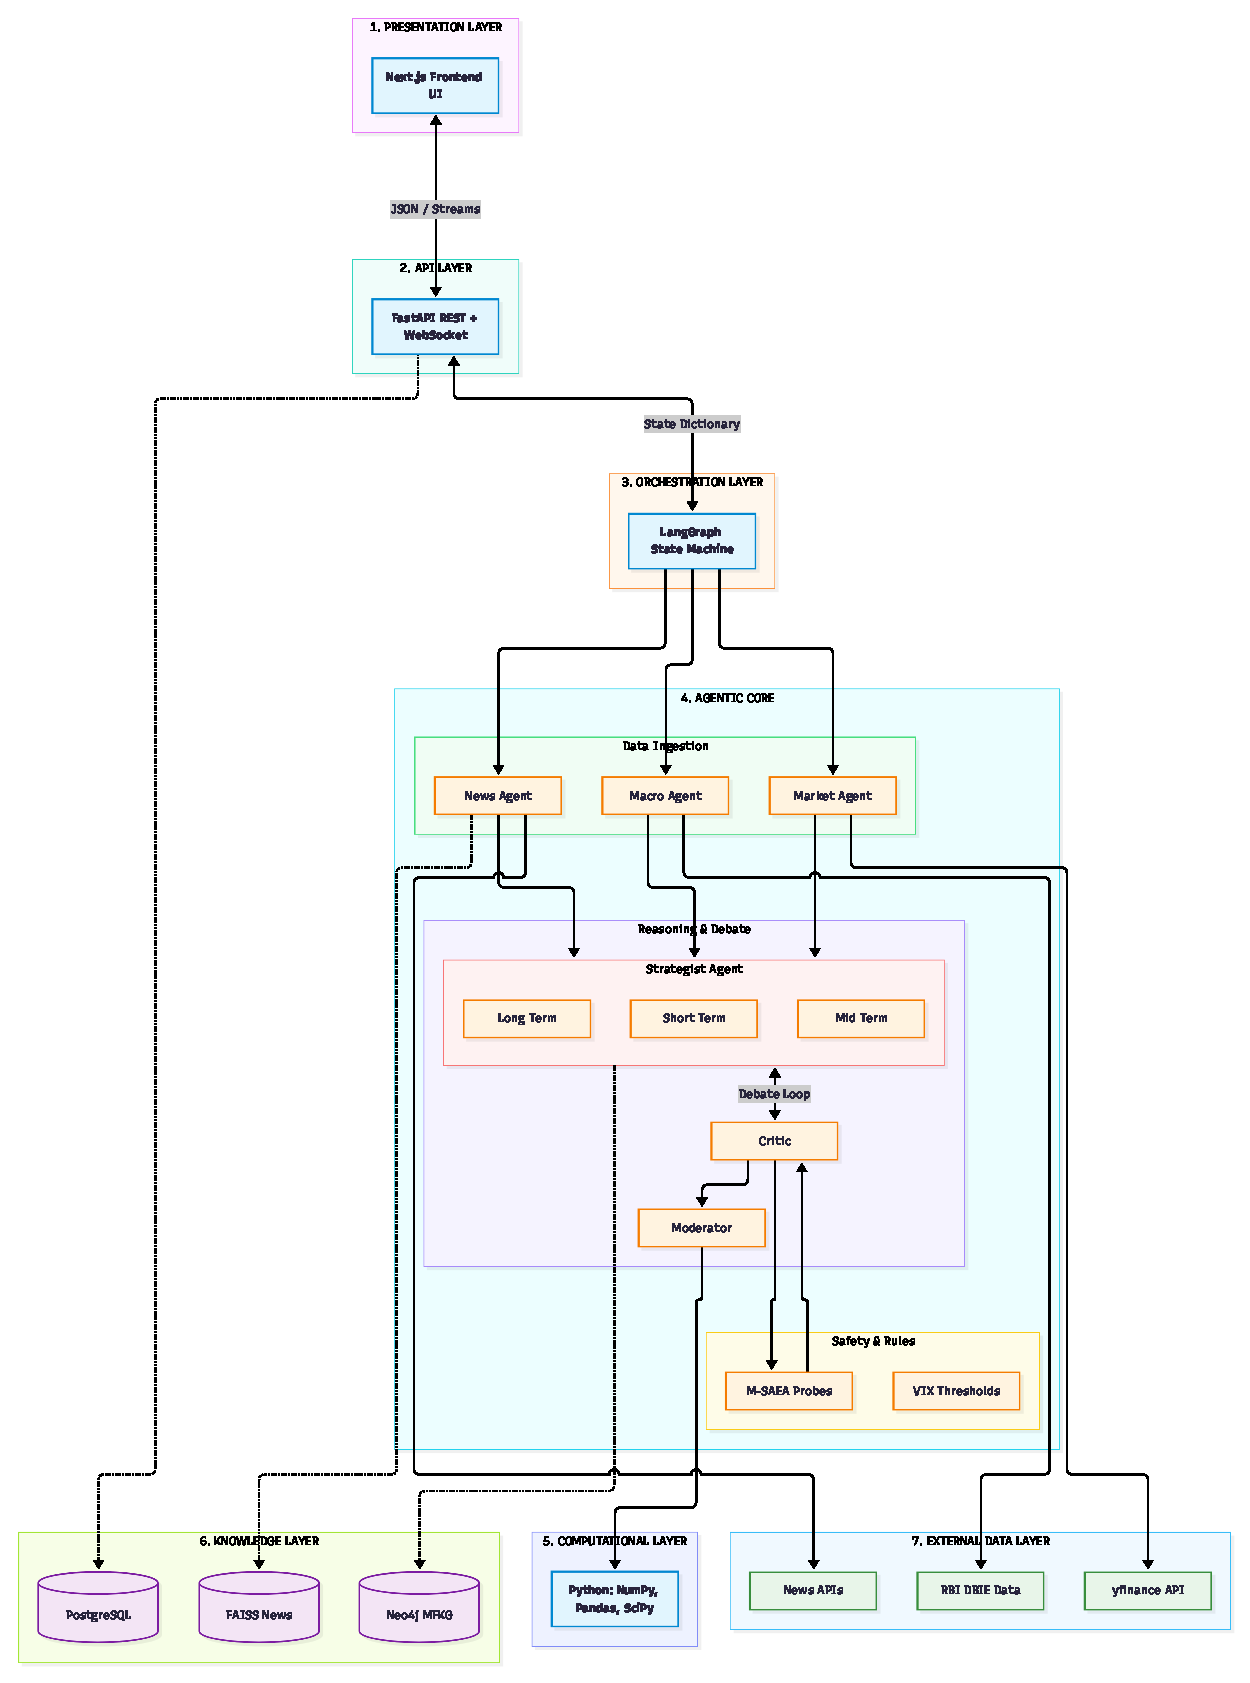
\includegraphics[width=\textwidth]{architecture.pdf}
    \caption{Detailed System Methodology and Agentic Pipeline}
    \label{fig:methodology}
\end{figure}

% =====================================================================
%  CHAPTER 6: DATA AND API REQUIREMENTS
% =====================================================================
\chapter{Data and API Requirements}

This chapter details the specific APIs and data sources required to build the application, based on the September 2026 API Research (Indian\_Portfolio\_API\_Data\_Complete\_2026\_v2).

\section{API Strategy and Selection}

The core principle for data acquisition is to use free, robust APIs for the student prototype (V1) while architecting the system so that production-grade commercial feeds can be hot-swapped later without changing the AI reasoning layer. 

The primary market data provider selected is \textbf{Upstox}, because its current Analytics Token is free, read-only, valid for one year, and covers market data, historical candles, fundamentals, and news.

\subsection{Primary API Stack (Prototype)}

\begin{table}[H]
\centering
\caption{Recommended API Stack for V1 Prototype}
\label{tab:api_stack}
\begin{tabularx}{\textwidth}{|l|X|X|}
\hline
\textbf{Category} & \textbf{Primary API / Source} & \textbf{Backup Alternative} \\
\hline
Current Prices \& Historical & Upstox (Analytics Token) & Dhan / Angel One SmartAPI \\
Company Fundamentals & Upstox Fundamentals API & CMIE Prowess (Academic) \\
India Market \& Macro & RBI DBIE (Data Portal) & MOSPI / NSE Website \\
Global Macro & FRED API (120 req/min limit) & World Bank Open Data \\
Financial News & Upstox News API & GNews / NewsAPI (Free tiers) \\
Mutual Fund Data & AMFI NAVAll (Public Feed) & MFKG internal database \\
AI Reasoning Engine & Gemini API (generateContent) & OpenAI (paid) \\
\hline
\end{tabularx}
\end{table}

\section{Operational Guidelines and Limits}

\subsection{Calculations to Perform Locally}
To minimise API costs and latency, the system shall \textbf{not} use paid APIs for derived metrics. The application will fetch raw OHLCV prices and compute the following locally in Python:
\begin{itemize}
    \item \textbf{Volatility and Beta}
    \item \textbf{Sharpe and Sortino Ratios}
    \item \textbf{Value at Risk (VaR) and Maximum Drawdown}
    \item \textbf{Moving Averages and Technical Indicators}
\end{itemize}

\subsection{API Rate Limits and Delays}
The application must handle the following operational limits gracefully:
\begin{itemize}
    \item \textbf{Upstox:} Standard REST limits apply (50 requests/sec, 500/min). Full Market Quotes V3 supports up to 500 instrument keys in a single request.
    \item \textbf{FRED API:} Returns HTTP 429 after 120 requests/minute.
    \item \textbf{News APIs (GNews/NewsAPI):} Free tiers have severe limitations (e.g., 100 requests/day, 12-to-24 hour delays). These should only be used as backups to Upstox News.
\end{itemize}

\section{Production Reality Check and Licensing}

A critical finding from the API research is that \textbf{technical access does not equal commercial redistribution rights}. 

While APIs like Upstox, Dhan, or free global providers (Twelve Data, EODHD) provide easy technical access to NSE/BSE data, their free tiers are strictly for non-commercial or internal use. Before moving from a student prototype to a public application, the system must integrate licensed data feeds.

\textbf{Production Replacements:}
\begin{itemize}
    \item \textbf{Real-time / Delayed Market Data:} NSE Data \& Analytics licensed product endpoints (e.g., the 15-minute delayed data tariff) or BSE Self Data Feed.
    \item \textbf{Commercial Display:} Requires explicit exchange agreements and payment of redistribution fees.
\end{itemize}

\section{Competitor Disclosure Patterns}

The lack of transparency in data sources is a major market gap. Table~\ref{tab:disclosure} documents what competitors reveal versus what they hide.

\begin{table}[H]
\centering
\caption{Competitor Data Disclosure Pattern (September 2026)}
\label{tab:disclosure}
\begin{tabularx}{\textwidth}{|X|l|}
\hline
\textbf{Information Area} & \textbf{Disclosure Level} \\
\hline
Market and fundamental data types used & Usually disclosed \\
News and macro data usage & Often disclosed \\
Portfolio and user data handling & Usually disclosed \\
Exact commercial data vendor & \textbf{Often NOT disclosed} \\
Exact factor formula or optimiser & \textbf{Often NOT disclosed} \\
Exact model architecture & \textbf{Usually NOT disclosed} \\
Training dataset and model weights & \textbf{NOT disclosed by any competitor} \\
\hline
\end{tabularx}
\end{table}

Our application addresses this pattern directly through the \textbf{Data Provenance (FR-D07)} feature, ensuring the user always knows the exact source, timestamp, and quality of the data driving their portfolio.

% =====================================================================
%  CONCLUSION
% =====================================================================
\chapter*{Conclusion}
\addcontentsline{toc}{chapter}{Conclusion}

This report has presented a comprehensive Functional Requirements Specification for an Agentic AI application for intelligent portfolio creation for the Indian retail investor market.

The competitive analysis of seven platforms (September 2026) confirms that features such as risk profiling, personalised portfolios, rebalancing, and AI-based stock analysis are already common and cannot serve as differentiators alone.

The genuine market opportunity lies in building the first integrated, transparent advisory workflow in India that connects the investor's goals to data, data to reasoning, reasoning to validated mathematics, and mathematics to a fully explained portfolio -- making every step of this chain visible and understandable to the investor.

The four most strategically powerful differentiating requirements are:

\begin{enumerate}
  \item \textbf{FR-D01 -- Reasoning Trace:} Per-stock, per-weight explanation in plain English.
  \item \textbf{FR-D02 -- Transparent Critic:} Showing the internal safety debate, not just the final answer.
  \item \textbf{FR-D03 -- LLM-Math Decoupling:} Structurally preventing AI hallucinations in portfolio calculations.
  \item \textbf{FR-D04 -- Regime-Aware Context:} Grounding AI decisions in verified historical expert behaviour.
\end{enumerate}

Together, these twenty requirements define an application built on the principle that an \textbf{informed investor is a better investor}. The goal is not to replace human judgment -- it is to make the AI's judgment fully understandable to the human who must ultimately decide to invest their money.

\end{document}
